\documentclass[10pt,twocolumn,letterpaper]{article}

\usepackage{cvpr}
\usepackage{times}
\usepackage{epsfig}
\usepackage{graphicx}
\usepackage{amsmath}
\usepackage{amssymb}
\usepackage{tikz}
\usepackage{pgfplots}

\usepackage{subcaption}

\usepackage{booktabs}

% Include other packages here, before hyperref.

% If you comment hyperref and then uncomment it, you should delete
% egpaper.aux before re-running latex.  (Or just hit 'q' on the first latex
% run, let it finish, and you should be clear).
\usepackage[breaklinks=true,bookmarks=false]{hyperref}

\cvprfinalcopy % *** Uncomment this line for the final submission

\def\cvprPaperID{****} % *** Enter the CVPR Paper ID here
\def\httilde{\mbox{\tt\raisebox{-.5ex}{\symbol{126}}}}
%\pgfplotsset{compat=1.14}
\pgfplotsset{compat=1.10}

% Pages are numbered in submission mode, and unnumbered in camera-ready
%\ifcvprfinal\pagestyle{empty}\fi
\setcounter{page}{1}
\begin{document}

%%%%%%%%% TITLE
\title{Error Correction for Optical Character Recognition via Language Models}

\author{Andrew Titus (\texttt{atitus}; 6.869), Brian Wheatman (\texttt{wheatman}; 6.869)\\
Massachusetts Institute of Technology\\
77 Massachusetts Avenue, Cambridge, MA 02139\\
{\tt\small \{atitus, wheatman\}@mit.edu}
% For a paper whose authors are all at the same institution,
% omit the following lines up until the closing ``}''.
% Additional authors and addresses can be added with ``\and'',
% just like the second author.
% To save space, use either the email address or home page, not both
}

\maketitle
%\thispagestyle{empty}

%%%%%%%%% ABSTRACT
\begin{abstract}
TODO
\end{abstract}

%%%%%%%%% BODY TEXT
\section{Introduction}
\label{introduction}
Optical character recognition (OCR) is one of the oldest problems
in computer vision. The process of determining the characters
contained within an image has been researched since the
19\textsuperscript{th} century \cite{Eikvil93-OCR} long before the
development of computers, starting with C.R. Carey's retina
scanner system in 1870. With the rise of convolutional neural networks,
however, modern-day OCR systems now exceed human-level performance on
standard OCR tasks \cite{Chen15-BHR}.

If we have exceeded human-level performance for OCR systems, why should we
continue to care about the task? One reason is that deep neural networks
can be easily fooled -- sometimes, it only takes a change of one pixel
to cause a network to incorrectly classify an image \cite{Su17-OPA}.
If the change of a single pixel can potentially cause a neural
network-based OCR model to incorrectly classify a character, then
the system can potentially make character-level errors that propagate
into word-level errors that can fundamentally change the meaning of
a sentence or make it unintelligible. This motivates the need for
robust OCR systems that can recover any character-level errors made
by neural-based models. Moreover, with millions of parameters in modern
computer vision systems \cite{AlexNet, VGG}, it can be too memory-
and/or computation-intensive to run such models in mobile or low-power
settings. In such settings, it can be desirable to have a simpler model
whose errors can be recovered.

In this paper, we evaluate the feasibility of using language
models to recover errors made by modern OCR models.  We do this
by training a simple OCR model and then trying to improve the
accuracy by post-processing the result with character-level
bigram language models. The probabilities computed in these language
models are then used in graphical Markov models to correct errors by
determining the most likely character sequences.

The rest of this paper is organized as follows. Related work is
discussed in Section \ref{related_work}, followed by a
description of our experimental setup in Section \ref{exp_setup}.
We then introduce our methods for error correction in Section 
\ref{error_correction} and describe related results in
Section \ref{exp_results}. Finally, we conclude the paper and
discuss future work in Section \ref{conclusion_future_work}.

\subsection{Individual Contribution: AUTHOR NAME}
\label{individual_contribution}
TODO



\section{Related Work}
\label{related_work}

Interest in correcting errors in the output of OCR systems began as
early as 1975 \cite{Neuhoff75-TVA}, where English text is treated as
a Markov source and maximum \textit{a posteriori} (MAP) estimation
is performed via the Viterbi algorithm \cite{Forney73-TVA} determine
the most likely sequence of characters. Hanson \textit{et. al.}
showed in 1976 that binary $n$-grams (bigrams) can significantly
reduce the word error rate (WER) of text recognition systems
\cite{Hanson76-CIW}, whereas Pollock and Zamora showed in
1984 that dictionary-based spelling error correction systems
can recover $65-80\%$ of misspellings in scientific texts
\cite{Pollock84-ASC}. Additionally, Tong and Evans showed
that OCR systems can reduce their word error rate by $60.2\%$
by using the Viterbi algorithm with word-bigram probabilities, and
can even self-calibrate by using the learned confusion probabilities
for specific OCR environments \cite{Tong96-ASA}.

This prior research on lexical error correction has been successfully
implemented in more recent systems. Bissacco \textit{et. al.} from
Google developed an OCR system (``PhotoOCR'') in 2013 with record
performance on standard OCR tasks (such as Street View Text, ICDAR, etc.)
by combining deep neural network character classifiers with large,
distributed $n$-gram models \cite{Bissacco13-PRT}. Additionally, 
PhotoOCR was optimized for usage on mobile devices for memory and
latency, with a reported mean processing time of 600 milliseconds.



\section{Experimental Setup}
\label{exp_setup}

For text data, we chose the King James Version of the Bible, a
common text corpus in natural language processing. We then
generated $352 \times 672$ pixel images with 32 rows
of 32 characters arranged in a grid using 18 point Andal\'{e}
Mono monospace font. Due to the size of the King James Version of
the Bible (several million characters and therefore several thousand
images) and time constraints for the project, we decided to use a
subset of the dataset, the Book of Genesis, which resulted in 200 images
and approximately 200,000 character examples.

We used our local machine for training and evaluating models,
which had a NVIDIA GeForce GT 740M Graphics with 2048MB of memory.
All models and analysis code were developed in Python, with the
neural network-based models being implemented in PyTorch with CUDA
GPU support.



\section{Error Correction}
\label{error_correction}
As shown in Section \ref{related_work}, many OCR systems exhibit significant
decreases in both character error rate (CER) and word error rate (WER)
when language modeling techniques are applied to the outputs of an OCR
model. In this paper, we investigate a simple language model --
character-level bigrams -- and evaluate its performance in reducing CER
and WER with two different error correction methods.

\subsection{Character Bigram Language Model}

A character bigram is defined as two characters that are adjacent to
each other in a given text sequence. The generalization of a bigram,
the $n$-gram, is used in language modeling to determine conditional
probabilities for a token given the previous $(n - 1)$ tokens (the
formula for a bigram is given in Equation \ref{bigram_eq}).
Character-level $n$-grams are a logical choice for a language model
in an OCR error correction task because OCR systems fundamentally act
at the character level by classifying individual characters. However,
when compared to word-level $n$-grams, these probabilities are much
more localized and do not effectively represent word distribution,
sentence structure and other information that can be useful in correcting
word-level errors (and thus improving word error rate).

\begin{equation}
\label{bigram_eq}
P(W_n|W_{n-1}) = \frac{P(W_{n-1}, W_{n})}{P(W_{n-1})}
\end{equation}

We chose bigrams specifically because they are memory-efficient and
are easily incorporated into graphical Markov models. Formally, for
a text dataset containing $C$ unique characters, a bigram model
needs only $\Theta(C^2)$ space, whereas $n$-grams use
$\Theta(C^{n})$ space (although this can
be relatively small in practice for larger $n$ due to sparsity from
$n$-grams with no occurrences in the dataset). Additionally, $n$-grams
are used for the transition probabilities in
$(n-1)$\textsuperscript{th} order Markov models.
Higher-order Markov models are infrequently used due to their high
computational cost and necessity for specialized extensions of algorithms
for first-order Markov models \cite{DuPreez98-ETO}, so the choice of
$n$ for which the most efficient Markov model decoding techniques exist
is 2, which corresponds to bigrams.

\begin{figure}
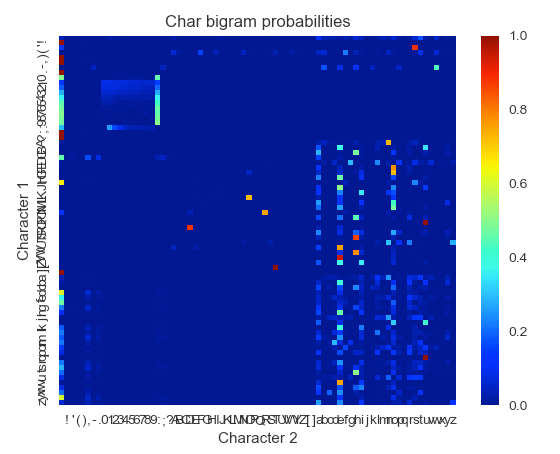
\includegraphics[scale=.45]{24272959_889664494543135_1476429274_n.png}
\caption{Heatmap of character bigram probabilities}
\label{fig:bigram_heatmap}
\end{figure}

We also observed two interesting trends in the character bigram probabilities shown in Figure \ref{fig:bigram_heatmap}
that could be potentially exploited by the model during error correction.
The first is an empirical verification of Benford's Law (also known as
the Significant-Digit Law) \cite{Hill95-ASD}. The Significant Digit Law states
that in many real-life distributions of numbers, the digits 1--9 appear less
frequently as the digit grows larger, with the digit 1 appearing about
$30\%$ of the time. Indeed, we see such a distribution for the King James
Version of the Bible in the upper left corner of this heatmap! The
second observation is that there are three significant outliers in the
capital letter to capital letter section of the bigram probabilities:
$P(O | L)$, $P(R | O)$, and $P(D | R)$. This is due to the fact that every
mention of ``the Lord'' is stylized as ``the LORD'' in this version of the
Bible.

\subsection{Noise Model}
Our noise model simulates having a data set which has ``smudges'' (i.e.,
occasional blurry images) in it. For our training set, we use raw images and
then test on data that has been degraded by adding a random value to each
pixel. This value is drawn from a zero mean Gaussian distribution with
varying standard deviation ($\sigma$).  In Figure \ref{fig:e_images}, one can see
images of the letter ``e'' that has had noise added to it. One can see
that for low levels of noise (under $\sigma = 0.5$), a human can easily
determine the true character label; however, for higher levels of noise,
it can be difficult for even humans to determine the true character label.
To simulate smudging, we only add the noise to a random subset of the images.

\begin{figure}
    \centering
    \begin{subfigure}[b]{0.22\textwidth}
        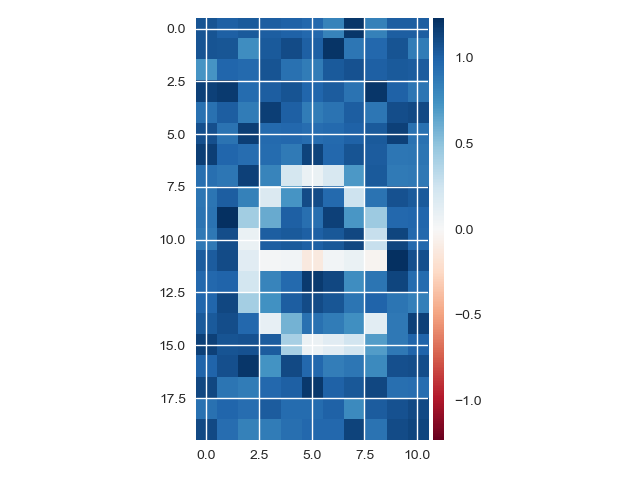
\includegraphics[width=\textwidth]{10.png}
        \caption{$\sigma = 0.1$}
    \end{subfigure}
    ~ %add desired spacing between images, e. g. ~, \quad, \qquad, \hfill etc. 
      %(or a blank line to force the subfigure onto a new line)
    \begin{subfigure}[b]{0.22\textwidth}
        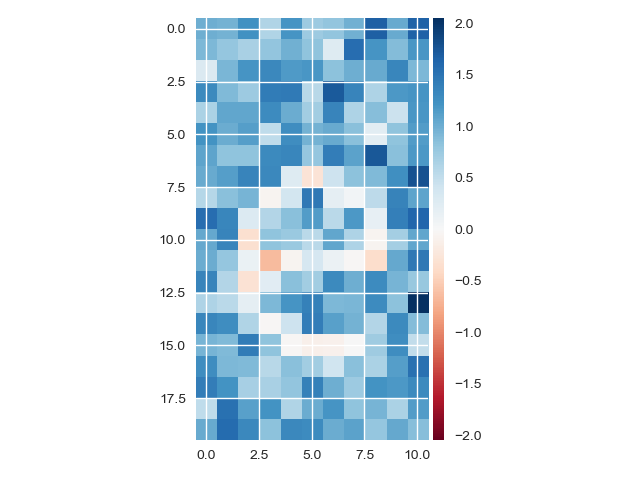
\includegraphics[width=\textwidth]{30.png}
        \caption{$\sigma = 0.3$}
    \end{subfigure}
    ~ %add desired spacing between images, e. g. ~, \quad, \qquad, \hfill etc. 

    \begin{subfigure}[b]{0.22\textwidth}
        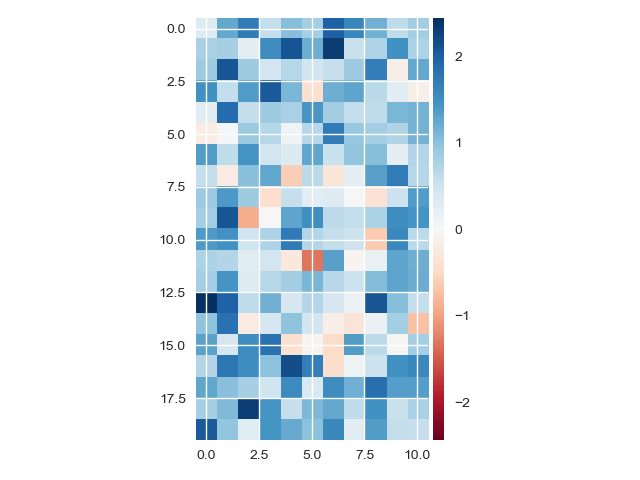
\includegraphics[width=\textwidth]{60.png}
        \caption{$\sigma = 0.6$}
    \end{subfigure}
    ~ %
    \begin{subfigure}[b]{0.22\textwidth}
        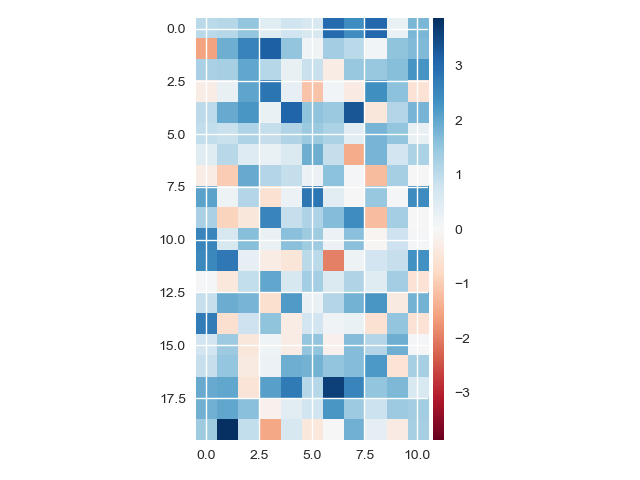
\includegraphics[width=\textwidth]{100.png}
        \caption{$\sigma = 1.0$}
    \end{subfigure}
    \caption{\label{fig:e_images} Additive Gaussian error on the letter ``e'' with varying standard deviation $\sigma$}
\end{figure}

\subsection{Text as Probabilistic Graphical Model}

Next, we define the probabilistic graphical model that will be used
for the error correction methods (see Figure
\ref{fig:probabilistic_graphical_model}. Let $G = (V, E)$ be a directed
Markov chain with $V = \text{length of dataset in characters}$ hidden
states. The edge weights from vertex $i$ to $j$ are simply the
character-level bigram probabilities $P(j | i)$, whereas the emission
probabilities $\Phi(i)$ are simply the normalized probabilities output
by the OCR model. In this model, we let the emission symbols equal the
hidden states, so emission probabilities are ignored.

\begin{figure}
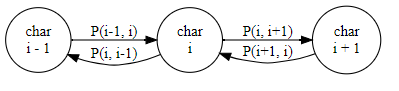
\includegraphics[scale=.8]{Capture.PNG}
\caption{\label{fig:probabilistic_graphical_model} Probabilistic graphical model for character-level error correction}
\end{figure}

\subsection{Belief Propagation}

One technique that we experimented with for correcting character-level
smudging errors is belief propagation. Belief propagation is a technique
that computes marginal probabilities for each state in a Markov chain
by passing ``messages'', which are simply partial sums from marginal
probability calculations of neighboring states that can be reused,
rather than recomputed. Formally, the marginal probability
of state $i$ being character $j$ is the product of incoming messages
$m_{i-1, i}$ and $m_{i + 1, i}$ from its neighbors $(i - 1)$ and
$(i + 1)$, respectively, or:
\begin{equation}
\begin{split}
P_i(x_j) &= \Phi_i(x_j) * m_{i - 1, i}(x_j) * m_{i + 1, i}(x_j) \\
&= \Phi_i(x_j) \left(\sum_{x_k} P(x_i | x_k) m_{i - 2, i - 1}(x_k) \right) *\\
&\hspace{15mm} \left(\sum_{x_k} P(x_k | x_i) m_{i + 1, i + 2}(x_k) \right) \\ 
\end{split}
\end{equation}

These messages are computed with a synchronous parallel update schedule,
where messages $m_{2, 3}(x_j), \cdots m_{N - 1, N}(x_j)$ are computed in
the increasing direction with boundary condition
$m_{1, 2}(x_j) = \Phi_1(x_j) \sum_{x_k} P(x_k | x_j)$ at the same time that
messages $m_{N - 1, N - 2}(x_j), \cdots m_{2, 1}(x_j)$ are computed in
the decreasing direction with boundary condition
$m_{N, N - 1}(x_j) = \Phi_N(x_j) \sum_{x_k} P(x_j | x_k)$.

The computational complexity of computing marginal probabilities for
$N$ nodes with $d$ possible states is thereby reduced from $O(d^N)$
(na\"{i}ve solution with recomputed messages) to $O(Nd^2)$ with
belief propagation (reusing messages). For OCR models, $d$ is
generally small (the number of unique characters) whereas $N$
can be on the order of millions of characters. Therefore, belief
propagation turns this intractable probability calculation into
something manageable on most computers.

\subsection{Viterbi Algorithm}

TODO



\section{Experimental Results}
\label{exp_results}
We first notice that in this constrained environment of only using the same mono-space font and not varying the text size that our simply linear model is able to get very high accuracy.  Furthermore as can be seen in Figure \ref{fig:CER} the model is able to determine the correct character under levels of noise that would make it difficult for humans.  In fact even when $\sigma = .1$ which as can be seen in Figure \ref{fig:e_images} is unintelligible, the model is able to correctly determine the letter about 65\% of the time. 

\begin{figure}
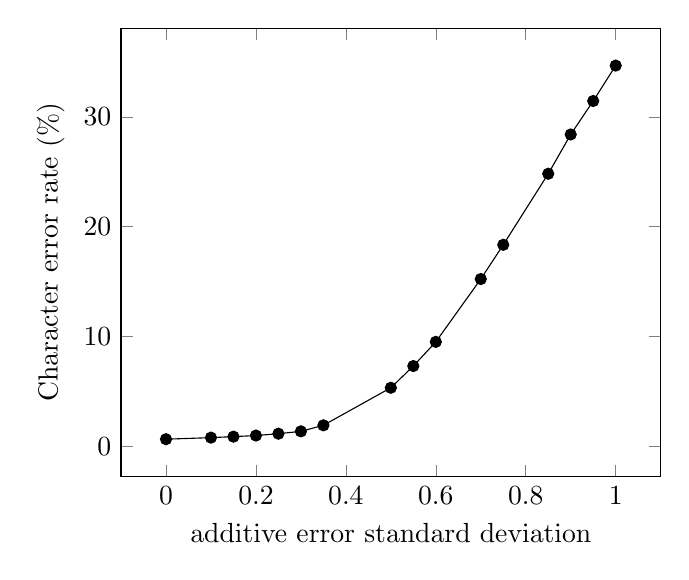
\begin{tikzpicture}
\begin{axis}[
    xlabel={additive error standard deviation},
    ylabel={Character error rate (\%)},
    legend pos=north west
]
\addplot[
    color=black,
    mark=*,
    ]
    coordinates {
    (0,.661)(.1,.803)(.15,.892)(.2,.993)(.25,1.16)(.3,1.374)(.35,1.924)(.5,5.341)(.55, 7.319)(.6, 9.517)(.7, 15.237)(.75, 18.352)(.85, 24.817)(.9, 28.393)(.95, 31.44)(1, 34.662)
    };
\end{axis}
\end{tikzpicture}
\caption{\label{fig:CER}How the CER changes with added noise to every image}
\end{figure}

For each of our runs we calculate a confusion matrix.  This is a matrix $M$ where $M[i][j]$ is the percent of the time that when $i$ was the true value that the model predicted $j$.  Figure \ref{fig:confusion} shows a confusion matrix with relatively high amount of noise, we can still almost always determine most of the characters, and the ones that are hard to determine are characters which appear very few times so they are not learned very well and unlikely to be guessed randomly, which might happen under high noise. 

\begin{figure}
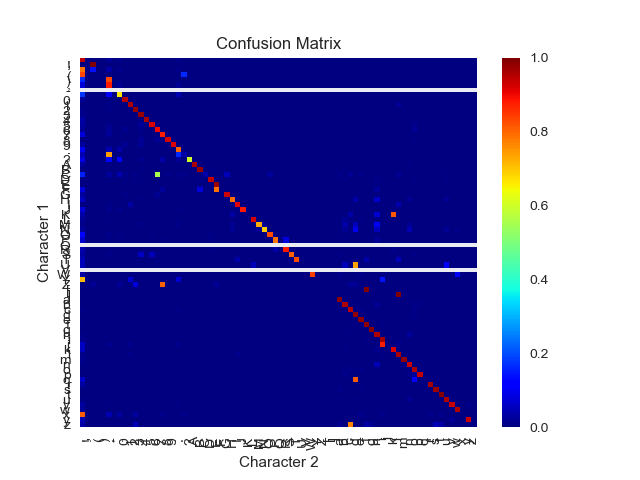
\includegraphics[scale=.5]{confusion.png}
\caption{\label{fig:confusion}This is a confusion matrix when we add noise to half of the images with standard deviation = .6}
\end{figure}


\subsection{error correction}
Our results are fixing the noised images were discouraging.  We added noise to 20\%, 30\%,and 40\% of the images with standard deviations between .4 and .5 since this was the point were images start being difficult for humans to determine the true labeling.  This gave us CER around 3-7\% and WER between 10 and 20\%.  After trying to fix it with both models the CER went up and for belief propagation the WER also went up.  the Viterbi algorithm was able to decrease the WER, however, it would only do so by about .1\%.  Overall this method seems like it will work, but more complete language models would be needed to significantly improve the performance.



\section{Conclusion and Future Work}
\label{conclusion_future_work}
While not as much as an improvement as we would have hoped we have shown that under certain conditions you can improve the accuracy of OCR by using language modeling.  This could be extended in many ways.  The first is using more elaborate language models.  Such as using n-grams and not just bigrams or using a word level model.  We could also test using a different base OCR model.  The goal is simplicity and performance in this case so it might be possible that you do not even need a full linear classifier and it can instead be even smaller.  Lastly we would hope to be able to use this on more different types of data, such as different fonts, size, and even hand written text.




{\small
\bibliographystyle{ieee}
\bibliography{egbib}
}

\end{document}